\usetikzlibrary{angles,quotes,decorations.pathreplacing}
% First draft: 1958_sichuan_q5_solution_fig1 (60-degree isosceles trapezoid, schematic scale).
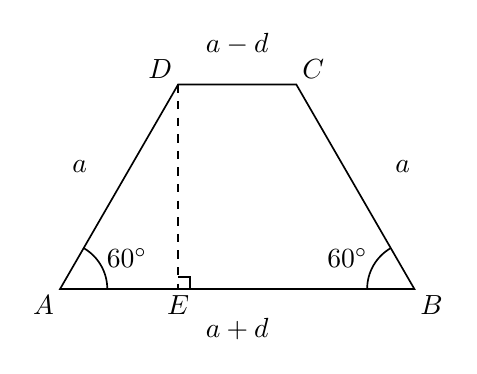
\begin{tikzpicture}[x=1cm,y=1cm,font=\normalsize,
 geometry edge/.style={solid,line width=.6pt},
 geometry mark/.style={solid,line width=.6pt},
 geometry label/.style={font=\normalsize,inner sep=2pt}]
\coordinate (A) at (0,0);
\coordinate (B) at (4.500000000,0.000000000);
\coordinate (D) at (1.500000000,2.598076211);
\coordinate (C) at (3.000000000,2.598076211);
\coordinate (E) at (1.5,0);
\coordinate (L_a1) at (0.42,1.55);
\coordinate (L_a2) at (4.180000000,1.550000000);
\coordinate (L_top) at (2.250000000,2.898076211);
\coordinate (L_bot) at (2.250000000,-0.300000000);
\coordinate (L_60A) at (0.850000000,0.400000000);
\coordinate (L_60B) at (3.650000000,0.400000000);
\coordinate (L_h) at (1.700000000,1.150000000);
\draw[geometry edge] (A)--(B)--(C)--(D)--cycle;
\draw[geometry edge,dashed] (D)--(E);
\pic[draw,line width=.6pt,angle radius=6mm] {angle=E--A--D};
\pic[draw,line width=.6pt,angle radius=6mm] {angle=C--B--A};
\node[geometry label,below left] at (A) {$A$};
\node[geometry label,below right] at (B) {$B$};
\node[geometry label,above right] at (C) {$C$};
\node[geometry label,above left] at (D) {$D$};
\node[geometry label,below] at (E) {$E$};
\node[geometry label,left] at (L_a1) {$a$};
\node[geometry label,right] at (L_a2) {$a$};
\node[geometry label,above] at (L_top) {$a-d$};
\node[geometry label,below] at (L_bot) {$a+d$};
\node[geometry label] at (L_60A) {$60^\circ$};
\node[geometry label] at (L_60B) {$60^\circ$};
\draw[geometry mark] (1.5,.15)--(1.65,.15)--(1.65,0);
\end{tikzpicture}
